\documentclass[10pt]{article}
\usepackage{enumitem}
\usepackage{graphicx}
\usepackage{subcaption}
\setlist[enumerate,1]{label=\textbf{\arabic*.}}
\setlist[enumerate,2]{label=\textbf{\alph*.}}
\usepackage[vmargin = 1.5cm, hmargin = 1.5cm]{geometry}
\usepackage{amsmath}
\title{\textbf{Projet Inpainting (4IM01) : Rapport intermédiaire}}
\author{Daniel Akbarinia \& Abdennour Kerboua}



\begin{document}

\maketitle

\section{Avancement}
L'inpainting basé sur des exemples (exemplar-based) est une méthode de restauration d'images qui remplit les zones manquantes d'une image en réutilisant les parties similaires de l'image intacte, permettant de conserver les textures et motifs visuels pour un résultat plus réaliste.
\\ L'article décrivant l'implémentation proposant un processus détaillé par étape, nous avons décidé de les suivre. Voici un résumé de notre état d'avancement sur chacune de ces étapes.

\begin{enumerate}
\item \begin{enumerate}
\item Identification du front de remplissage (noté $\delta \Omega^t$, dans l'article) : on a implémenté deux méthodes. La première consiste à maintenir à jour une matrice indiquant pour chaque pixel son état de remplissage (\verb+True+ pour rempli, \verb+False+ pour en attente de remplissage). A partir de cette matrice, on décide pour chaque pixel, s'il appartient au front de remplissage par 8-connexité (un pixel $p_{i,j}$ non rempli appartient à $\delta \Omega^t$ si et seulement si $\exists k,l \in [i-1,i+1] \times [j-1,j+1]$, tel que $p_{k,l}$ est rempli). La seconde est une variante équivalente qui convolue le masque (valant 1 en les pixels remplis et 0 autre part) avec le filtre : $\begin{pmatrix} 1 & 1 & 1 \\ 1 & 1 & 1 \\ 1 & 1 & 1  \end{pmatrix}$. En prenant l'intersection des pixels nuls dans l'image de départ et des pixels strictement positifs dans l'image résultante de la convolution, on obtient le front de remplissage.
\item Calcul des priorités : Ce calcul implique deux le calcul de deux facteurs : la confidence $C(p)$ et le terme \textit{data} $D(p)$,

\begin{itemize}
\item \textbf{Confidence} : On maintient à jour une matrice \verb+confidence+ de même taille que l'image qui contient pour chaque pixel $p_{i,j}$ la valeur de la confidence de ce pixel. Elle est initialisé en affectant 0 aux pixels de la zone cible et 1 à ceux de la zone source. Au début de chaque itération du programme, la priorité des pixels du contour actuel est calculé suivant cette formule : 
\begin{equation} C(p) = \frac{\sum_{q\in \Psi_p \cap \bar{\Omega} } C(q) }{|\Psi_p||} 
\label{confidence}
\end{equation} 

Ce terme permet de favoriser le remplissage en cercle concentrique.
\item \textbf{Coefficient \textit{Data}} : Il s'obtient à partir de cette formule : $D(p) = \frac{|\overrightarrow{\nabla I}^\perp \cdot \overrightarrow{n_p}|}{\alpha}$. Avec,
\begin{itemize}
\item  $\overrightarrow{n_p}$ : le vecteur normal au contour de remplissage au pixel $p$, on le calcule en prenant le gradient au point $p$ du masque (valant 0 au pixel non-rempli et 1 ailleurs)
\item $\overrightarrow{\nabla I}^\perp $ : l'orthogonal du vecteur gradient au point $p$. On explore actuellement plusieurs méthodes de calcul. La surface manquante étant noircie, un calcul usuel de différences au point $p$ peut donner lieu à des valeurs aberrantes. Si l'accès à l'image d'origine est possible (dans le cas d'une suppression volontaire) le calcul du gradient peut se faire sur cette dernière. Sinon, nous avons implémenté : \begin{itemize} \item un calcul moyennant le gradient sur les pixels de la zone rempli ne faisant pas intervenir les pixels de la zone noire (non-remplie) \item un calcul prenant le maximum du gradient sur les pixels de la zone rempli ne faisant pas intervenir les pixels de la zone noire (non-remplie)  \end{itemize}
Comme on utilise un filtre de Sobel pour calculer le gradient, pour éviter que les pixels noirs de la bordure influencent le gradient aux pixels voisins de la bordure, on remplace les pixels de la bordure par la moyenne des pixels remplis du patch. 
\end{itemize}
\end{itemize}
\end{enumerate}
\item \begin{enumerate}
\item On obtient alors le terme de priorité pour chaque pixel du contour et on accède facilement au pixel de plus grande priorité. On sauvegarde alors le patch cible $\Psi_p$ de taille fixé en début de programme (le plus souvent $9 \times 9$)
\item La fonction \verb+distance+ est implémenté de façon à renvoyer la SSD entre un patch $\Psi_t$ et un patch source $\Psi_s$ par des calculs élémentaires. On trouve alors le meilleur patch en parcourant tous les patchs de l'image et en retenant le patch $\Psi_s$ tel que la valeur \verb+distance(+$\Psi_p, \Psi_s$\verb+)+ est minimale. La recherche est l'étape la plus chronophage de l'algorithme. On expérimente alors des variantes limitant la recherche à un certain voisinage de la zone cible $\Omega$.
\item Etape triviale
\end{enumerate}
\item On met à jour la matrice \verb+priority+ avec la formule: $C(\mathbf{q}) = C(\hat{\mathbf{p}}) \quad \forall \mathbf{q} \in \Psi_{\hat{p}} \cap \Omega$.

\end{enumerate}

\section{Résultats}
\begin{figure}[h]
    \centering
    \begin{subfigure}{0.4\textwidth}
        \centering
        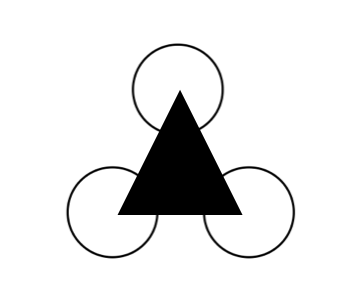
\includegraphics[width=\textwidth]{images/triangle.png}
        \caption{image masquée}
    \end{subfigure}
    \hfill
    \begin{subfigure}{0.4\textwidth}
        \centering
        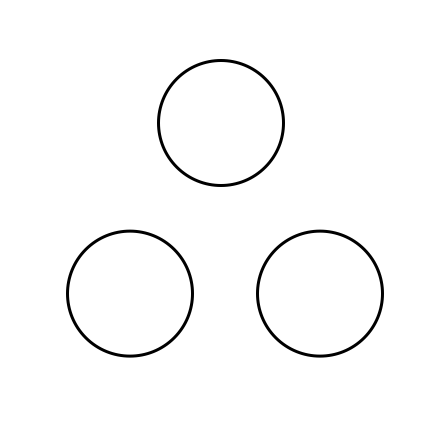
\includegraphics[width=\textwidth]{images/triangle_inpaint.png}
        \caption{image remplie avec l'algorithme}
    \end{subfigure}
    \caption{Comparaison des images côte à côte}
\end{figure}

\begin{figure}[h]
    \centering
    \begin{subfigure}{0.4\textwidth}
        \centering
        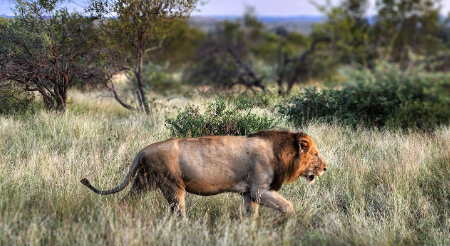
\includegraphics[width=\textwidth]{images/lion.png}
        \caption{image masquée}
    \end{subfigure}
    \hfill
    \begin{subfigure}{0.4\textwidth}
        \centering
        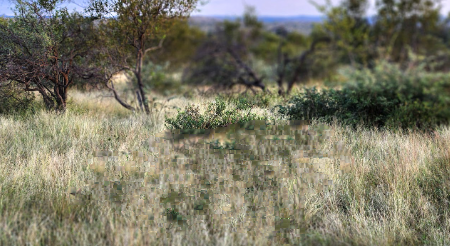
\includegraphics[width=\textwidth]{images/lion_inpaint.png}
        \caption{image remplie avec l'algorithme}
    \end{subfigure}
    \caption{Comparaison des images côte à côte}
\end{figure}

\begin{figure}[h]
    \centering
    \begin{subfigure}{0.3\textwidth}
        \centering
        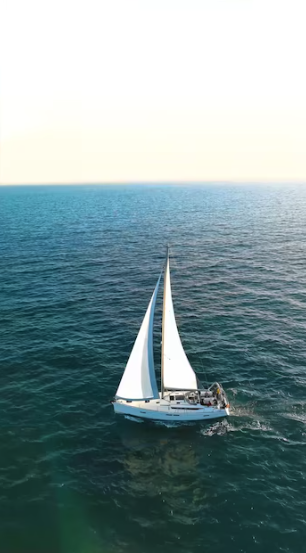
\includegraphics[width=\textwidth]{images/sailboat.png}
        \caption{Image masquée}
    \end{subfigure}
    \hspace{0.05\textwidth} 
    \begin{subfigure}{0.3\textwidth}
        \centering
        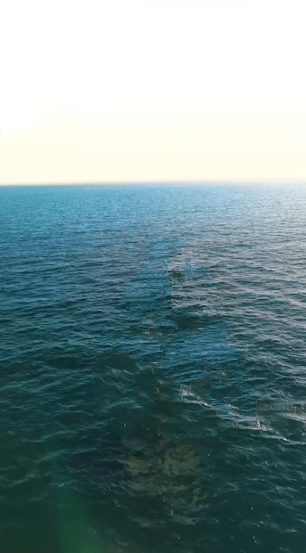
\includegraphics[width=\textwidth]{images/image_sailboat_inpaint.png}
        \caption{Image remplie avec l'algorithme}
    \end{subfigure}
    \caption{Comparaison des images côte à côte}
\end{figure}

\begin{figure}[h]
    \centering
    \begin{subfigure}{0.3\textwidth}
        \centering
        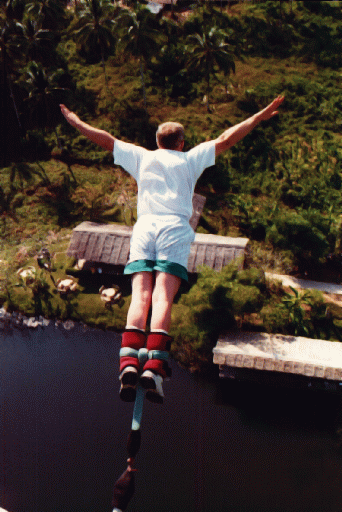
\includegraphics[width=\textwidth]{images/bungee.png}
        \caption{Image masquée}
    \end{subfigure}
    \hspace{0.05\textwidth} 
    \begin{subfigure}{0.3\textwidth}
        \centering
        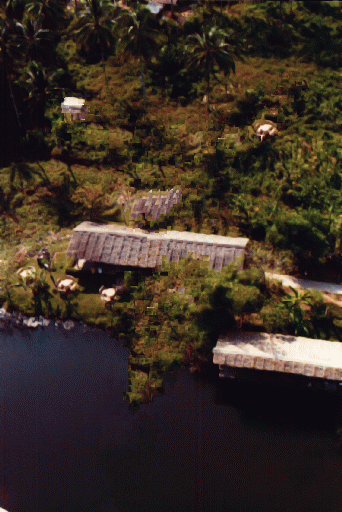
\includegraphics[width=\textwidth]{images/bungee_inpaint.png}
        \caption{Image remplie avec l'algorithme}
    \end{subfigure}
    \caption{Comparaison des images côte à côte}
\end{figure}

\end{document}